%===============================================================================
% main.tex
%
% Author: Robert Gaugl
%
% Content: This file loads all packages and document settings,
%          and calls the individual subchapters
%===============================================================================

%===============================================================================
% Metadata (AJUST!)
%===============================================================================

% Language Selection: Uncomment one to select the language (this will also adjust the title page
\newcommand{\documentlanguage}{english}
%\newcommand{\documentlanguage}{german}

\newcommand{\thesistype}{Master} % Change to "Bachelor" to adapt title page for Bachelor's thesis

\newcommand{\thesistitle}{Title of the Thesis} % Title of Thesis
\newcommand{\thesisauthor}{First Last Name} % Your name
\newcommand{\supervisor}{Supervisor Name} % Name of supervisor (Betreuer)
\newcommand{\reviewer}{Reviewer Name} % Only for Master's; Name of reviewer (Beurteiler)
\newcommand{\studyprogram}{Electrical and Electronics Engineering} % Name of study programme
\newcommand{\submissionmonth}{April} % Month
\newcommand{\submissionyear}{2025} % Year

%===============================================================================
% Document properties
% A4 paper size, left-aligned equations, header/footer lines, 12pt font
%===============================================================================
\documentclass[a4paper, fleqn, headsepline, footsepline, 12pt, parskip=half]{scrartcl}

% Define content area size
\areaset{16cm}{27cm}

%===============================================================================
% Load packages
%===============================================================================

% !TEX root = ./main.tex
%===============================================================================
% preamble.tex
%
% Author: Robert Gaugl
%
% Content: Contains all usepackage declarations and document settings
%===============================================================================

%===============================================================================
% If-then package
%===============================================================================
\usepackage{ifthen}

%===============================================================================
% Language and typography
%===============================================================================
\ifthenelse{\equal{\documentlanguage}{german}}{
    \usepackage[ngerman]{babel}       % German hyphenation and terms
}{
    \usepackage[english]{babel}       % English hyphenation and terms
}

\usepackage{csquotes}                 % Recommended with babel + biblatex
\usepackage{microtype}                % Improves typography: better kerning, protrusion, spacing
\usepackage{lmodern}                  % Improved font rendering

%===============================================================================
% Math and formatting
%===============================================================================
\usepackage{amsmath}                  % Advanced math features
\setlength{\mathindent}{1cm}          % Indentation of equations
\usepackage[onehalfspacing]{setspace} % Line spacing

% Prevent widows and orphans
\clubpenalty     = 10000
\widowpenalty    = 10000
\interlinepenalty= 10000

%===============================================================================
% Graphics and tables
%===============================================================================
\usepackage{graphicx}                 % Include images
\usepackage{float}                    % Precise figure placement
\usepackage{booktabs}
\usepackage{colortbl}
\usepackage{multirow}
\usepackage{hhline}
\usepackage{tabularx}
\usepackage{siunitx}
\ifthenelse{\equal{\documentlanguage}{german}}{
    \sisetup{
        output-decimal-marker = {,},  % use comma as decimal separator
        group-separator = {.},        % use dot as thousand separator
        group-minimum-digits = 4,     % format large numbers
        group-digits=integer
    }
}{
    \sisetup{
        output-decimal-marker = {.},  % use comma as decimal separator
        group-separator = {~},        % use space as thousand separator
        group-minimum-digits = 4,     % optional: format large numbers
        group-digits=integer
    }
}
\DeclareSIUnit \watthour { Wh } %apparent power 


%===============================================================================
% Chemistry and symbols
%===============================================================================
\usepackage[version=4]{mhchem}        % Chemical symbols
\usepackage{eurosym}                  % Euro symbol: \euro

%===============================================================================
% Colors and custom commands
%===============================================================================
\usepackage{xcolor}                   % Text colors
\definecolor{blue}{rgb}{0,0,1}        % Revision color
\newcommand{\rev}[1]{\textcolor{blue}{#1}}

%===============================================================================
% Hyperlinks and PDF metadata
%===============================================================================
\usepackage[pdfborder={0 0 0}]{hyperref}
\usepackage{url}
\PassOptionsToPackage{hyphens}{url}   % Allow line breaks in URLs

%===============================================================================
% Bibliography
%===============================================================================
\usepackage[
  backend      = biber,
  style        = ieee,
  sorting      = none,
  natbib       = true,
  hyperref     = true,
  maxbibnames  = 3,
  dashed       = false
]{biblatex}
\addbibresource{./Literature.bib}

\DefineBibliographyStrings{german}{
  andothers = {et al.}
}

% Avoid broken links in bibliography
\setcounter{biburlnumpenalty}{100}
\setcounter{biburlucpenalty}{100}
\setcounter{biburllcpenalty}{100}

%===============================================================================
% To-Do notes
%===============================================================================
\usepackage{todonotes}

%===============================================================================
% Sectioning and numbering
%===============================================================================
\setcounter{secnumdepth}{5}          % Depth of numbered sections
\setcounter{tocdepth}{3}             % Depth in table of contents

% Numbering equations by section
\makeatletter
  \@addtoreset{equation}{section}
  \renewcommand \theequation{\thesection.\arabic{equation}}
  \@addtoreset{figure}{section}
  \renewcommand \thefigure{\thesection.\arabic{figure}}
  \@addtoreset{table}{section}
  \renewcommand \thetable{\thesection.\arabic{table}}
\makeatother

%===============================================================================
% Custom environments
%===============================================================================
\newtheorem{Beispiel}{Example}[section]

%===============================================================================
% Utility commands
%===============================================================================
\usepackage{afterpage}
\newcommand{\blankpage}{
  \null
  \thispagestyle{empty}
  \addtocounter{page}{-1}
  \newpage
} % Load preamble with packages and settings

%===============================================================================
% Start of the actual document
%===============================================================================
\begin{document}
    %===========================================================================
    % Pre-content pages (front matter)
    %===========================================================================

    % Title page
    % !TEX root = ../main.tex
%===============================================================================
% A01_Title_page.tex
%
% Author: Robert Gaugl
%
% Content: Title page of the document
%===============================================================================

\pagestyle{empty}
\enlargethispage*{23cm}

% Define bilingual static text
\ifthenelse{\equal{\documentlanguage}{english}}{
    \ifthenelse{\equal{\thesistype}{Bachelor}}{
        \newcommand{\thesisdegree}{Bachlor's Thesis}
        \newcommand{\degreeinfoFull}{Bachelor of Science}
        \newcommand{\programinfo}{Bachelor's degree programme}
    }{
        \newcommand{\thesisdegree}{Master's Thesis}
        \newcommand{\degreeinfoFull}{Diplom-Ingenieur}
        \newcommand{\programinfo}{Master's degree programme}
    }
    \newcommand{\textone}{to achieve the university degree of}
    \newcommand{\texttwo}{submitted to}
    \newcommand{\universityinfo}{Graz University of Technology}
    \newcommand{\textthree}{Supervisor}
    \newcommand{\textfour}{Reviewer}
    \newcommand{\instituteinfo}{Institute of Electricity Economics and Energy Innovation}
    \newcommand{\submissiontext}{Graz, \submissionmonth~\submissionyear}
}{
    \ifthenelse{\equal{\thesistype}{Bachelor}}{
        \newcommand{\thesisdegree}{Bachelorarbeit}
        \newcommand{\degreeinfoFull}{Bachelor of Science}
        \newcommand{\programinfo}{Bachelorstudium}
    }{
        \newcommand{\thesisdegree}{Masterarbeit}
        \newcommand{\degreeinfoFull}{Diplom-Ingenieur}
        \newcommand{\programinfo}{Masterstudium}
    }
    \newcommand{\textone}{zur Erlangung des akademischen Grades}
    \newcommand{\texttwo}{eingereicht an der}
    \newcommand{\universityinfo}{Technische Universität Graz}
    \newcommand{\textthree}{Betreuer}
    \newcommand{\textfour}{Beurteiler}
    \newcommand{\instituteinfo}{Institut für Elektrizitätswirtschaft und Energieinnovation}
    \newcommand{\submissiontext}{Graz, \submissionmonth~\submissionyear}
}

%===============================================================================
% Calculate spaces between elements depending on length of title
\newdimen\height
\newdimen\spaceonedim
\newdimen\spacetwodim
\newdimen\tempdimen
\newdimen\tempdimentwo
\newcount\scalefactor

\setbox0=\vbox{\LARGE\textbf{\thesistitle}}
\height=\ht0 \advance\height by \dp0

% Step 1: \tempdimen = \height - 14.5949pt
\tempdimen=\height
\advance\tempdimen by -14.5949pt

% Step 2: scale \tempdimen by (192pt / 362pt) = approx 0.530387
% Since TeX can’t do floating point math, we use fixed-point integer math

% Let's use: (192000 / 362000), multiplying and then dividing
\tempdimen=\dimexpr \tempdimen * 192 / 362\relax
\tempdimentwo=\dimexpr \tempdimen * 170 / 362\relax

% Step 3: divide by 4
\tempdimen=\dimexpr \tempdimen / 3\relax
\tempdimentwo=\dimexpr \tempdimen / 4\relax

% Step 4: add 48pt
\spaceonedim=\dimexpr 48pt - \tempdimen\relax
\spacetwodim=\dimexpr 34pt - \tempdimentwo\relax

\newcommand{\spaceone}{\the\spaceonedim}
\newcommand{\spacetwo}{\the\spacetwodim}

%===============================================================================

\vspace*{-1.5cm}
\begin{center}
    
\includegraphics[width=3.3cm]{figures/TU_Graz_Logo.pdf}
    
    \vspace*{\spaceone}
    
    {\normalsize \textbf{\thesisauthor\\}}
    
    \vspace*{\spaceone} 
    \LARGE\textbf{\thesistitle}
    
    \vspace*{\spacetwo} 
    \large{\textbf{\thesisdegree\\}}
    
    \vspace*{\spacetwo}
    {\normalsize \textone\\}
    {\normalsize \degreeinfoFull\\}

    \vspace*{\spacetwo}{\normalsize \programinfo\\}
    {\normalsize \studyprogram\\}

    \vspace*{\spacetwo}{\normalsize \texttwo\\}
    \large{\textbf{\universityinfo\\}}
    
    \vspace*{\spaceone}\large{\textbf{\textthree\\}}
    {\normalsize \supervisor\\}

    % Only for Master's theses
    \ifthenelse{\equal{\thesistype}{Master}}{
      \large{\textbf{\textfour\\}} % Only for Master's
      {\normalsize \reviewer\\}
    }    
    
    \vspace*{\spacetwo}
    \normalsize \instituteinfo\\
    
    \vspace*{\spaceone}
    \small{\textbf{\submissiontext\\}}
    
\end{center}

\clearpage
    \blankpage

    % Disable headers and footers, use Roman page numbers for front matter
    \pagestyle{plain}
    \pagenumbering{roman}

    % Acknowledgements
    % !TEX root = ../main.tex
%===============================================================================
% A02_Acknowledgements.tex
%
% Author: Robert Gaugl
%
% Content: Acknowledgements
%===============================================================================

\ifthenelse{\equal{\documentlanguage}{german}}{
    \section*{Danksagung}
}{
    \section*{Acknowledgements}
}


Lorem ipsum dolor sit met, consetetur sadipscing elitr, sed diam nonumy eirmod tempor invidunt ut labore et dolore magna aliquyam erat, sed diam voluptua. At vero eos et accusam et justo duo dolores et ea rebum. Stet clita kasd gubergren, no sea takimata sanctus est Lorem ipsum dolor sit amet. Lorem ipsum dolor sit amet, consetetur sadipscing elitr, sed diam nonumy eirmod tempor invidunt ut labore et dolore magna aliquyam erat, sed diam voluptua. At vero eos et accusam et justo duo dolores et ea rebum. Stet clita kasd gubergren, no sea takimata sanctus est Lorem ipsum dolor sit amet. Lorem ipsum dolor sit amet, consetetur sadipscing elitr, sed diam nonumy eirmod tempor invidunt ut labore et dolore magna aliquyam erat, sed diam voluptua. At vero eos et accusam et justo duo dolores et ea rebum. Stet clita kasd gubergren, no sea takimata sanctus est Lorem ipsum dolor sit amet.

Duis autem vel eum iriure dolor in hendrerit in vulputate velit esse molestie consequat, vel illum dolore eu feugiat nulla facilisis at vero eros et accumsan et iusto odio dignissim qui blandit praesent luptatum zzril delenit augue duis dolore te feugait nulla facilisi. Lorem ipsum dolor sit amet, consectetuer adipiscing elit, sed diam nonummy nibh euismod tincidunt ut laoreet dolore magna aliquam erat volutpat.

Ut wisi enim ad minim veniam, quis nostrud exerci tation ullamcorper suscipit lobortis nisl ut aliquip ex ea commodo consequat. Duis autem vel eum iriure dolor in hendrerit in vulputate velit esse molestie consequat, vel illum dolore eu feugiat nulla facilisis at vero eros et accumsan et iusto odio dignissim qui blandit praesent luptatum zzril delenit augue duis dolore te feugait nulla facilisi.

Nam liber tempor cum soluta nobis eleifend option congue nihil imperdiet doming id quod mazim placerat facer possim assum. Lorem ipsum dolor sit amet, consectetuer adipiscing elit, sed diam nonummy nibh euismod tincidunt ut laoreet dolore magna aliquam erat volutpat. Ut wisi enim ad minim veniam, quis nostrud exerci tation ullamcorper suscipit lobortis nisl ut aliquip ex ea commodo consequat. 
    \newpage

    % Abstract
    % !TEX root = ../main.tex
%===============================================================================
% A03_Absctract.tex
%
% Author: Robert Gaugl
%
% Content: Abstract in German and English
%===============================================================================

\section*{Kurzfassung}

Max. 4.000 Zeichen inkl. Leerzeichen. Unbedingt einhalten, weil die Kurzfassung im weiteren Verlauf auch ins TUGonline hochgeladen werden muss und dort diese Grenze gilt.

Eine allgemeine Zusammenfassung über den Inhalt der Arbeit. Es soll sich nicht einfach um eine Zusammenfassung aller Kapitel handeln, sondern fasse kurz die Fragestellung der Arbeit zusammen und begründe warum es eine behandlungswürdige Fragestellung ist. Erkläre kurz wie du vorgegangen bist und gib eventuell auch einen kleinen Überblick über die Resultate deiner Arbeit.

\newpage

\section*{Abstract}

Maximum 4~000 characters including spaces. This limit must be strictly observed, as the abstract will also be uploaded to TUGonline later, where this restriction applies.

A general summary of the content of the thesis. It should not simply be a summary of all chapters, but briefly present the research question of the thesis and explain why it is a topic worthy of investigation. Briefly describe your approach and, if applicable, provide a short overview of the results of your work.




 

    \newpage

    % Table of contents
    % !TEX root = ../main.tex
%===============================================================================
% A04_Table_of_content.tex
%
% Author: Robert Gaugl
%
% Content: Table of content
%===============================================================================

% Table of Contents
\tableofcontents
\pagebreak
    \newpage

    %===========================================================================
    % Main content (body of the document)
    %===========================================================================

    % Enable headers/footers and switch to Arabic page numbers
    \pagestyle{headings}
    \pagenumbering{arabic}

    % Chapter: Introduction
    % !TEX root = ../main.tex
%===============================================================================
% B01_Introduction.tex
%
% Author: Robert Gaugl
%
% Content: Lorem Ipsum
%===============================================================================

\section{Introduction}
\label{sec:introduction}

This chapter aims to explain why your research question is of interest. In addition, general explanations regarding your thesis can be described here, or an overview of current technologies can be provided. A ToDo can be inserted with the command \textbackslash todo\{text\} \todo{This is a sample ToDo.}.


%===============================================================================
\subsection{Subchapter}
\label{sec:subchapter}

This is what a subchapter\footnote{Footnotes can be used to include details that are not important enough to be explained in the main text.} looks like.

To avoid a mess of numbering like {\glqq}1.2.1.3.4.5 Subchapter 5{\grqq}, use a maximum of three (1.2.3 heading) to four (1.2.3.4 heading) digits in the heading numbering. In the table of contents, only headings with up to three digits will be displayed.


%===============================================================================
\subsubsection{Figures}
\label{sec:figures}

Figure~\ref{fig:Baum} shows an example of an image with a suitable caption. Every figure must also be described and referenced in the text. For non-original images, don’t forget the source citation. If a figure is created by yourself but based on data from another source, that must be indicated as well (data from [XY] or based on [XY]).

\begin{figure}[H]
	\begin{center}
		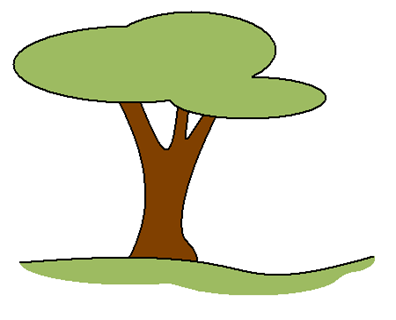
\includegraphics{figures/tree.png}
		\caption{This is a beautiful tree.}
		\label{fig:Baum}
	\end{center}
\end{figure}


%===============================================================================
\subsubsection{Tables}
\label{sec:tables}

The design of a table is up to the bachelor's/master's student. However, it should be clearly legible and, if possible, have a consistent design throughout the document.

If tables from the internet are used, they should be recreated and properly cited. Table~\ref{tab:Tabelle1} is an example of what a table might look like. Note how the numbers are neatly aligned at the decimal separator. This alignment is achieved using the siunitx package with the S[table-format=4.1] column specification, which in this case allows up to 4 digits before the comma and 1 digit after.

At our institute, there is no fixed rule whether the table caption should be above or below the table. However, as with figures: every table must be described and referenced in the text.

\begin{table}[H]
	\centering 
	\begin{tabular}{c S[table-format=1.1] S[table-format=1.0] S[table-format=2.2] S[table-format=4.1]}
		\hline
		\textbf{Scenarios} & \textbf{RAV [\%]} & \textbf{[\euro/MWh]} & \textbf{[Million \euro]} & \textbf{[\euro/MWh]} \\
		\hline
		\rowcolor[gray]{0.9}
		Scenario 1 & 0,5 & 5 & 10,24 & 14,9 \\
		Scenario 2 & 0,5 & 10 & 0,39 & 24,1 \\
		\rowcolor[gray]{0.9}
		Scenario 3 & 0,5 & 20 & 0,69 & 1042,8 \\
		Scenario 4 & 1,0 & 5 & 0,33 & 120,5 \\
		\hline \hline
	\end{tabular}
	\caption{This is a test table}\label{tab:Tabelle1}
\end{table}


%===============================================================================
\subsubsection{Equations}
\label{sec:equations}

Unlike figures and tables, equation numbering is placed on the right side. Unlike Microsoft Word, LaTeX handles this automatically.

The symbol for multiplication is achieved by typing '\textbackslash cdot' within the math environment. The commonly (and incorrectly) used '*' symbol stands for convolution, not multiplication!

Equation~\ref{eq:Ohmsches_Gesetz} shows an example of a correctly formatted formula with numbering and explanation of the variables.

\begin{align}
	\label{eq:Ohmsches_Gesetz}
	U &= R \cdot I
\end{align}
\vspace*{-1cm}
\begin{table}[H]
	\begin{tabular}{@{}p{1cm}@{}p{1cm}<{\dotfill}@{}p{\dimexpr\linewidth-5cm}}
		& $U$ & Voltage in $V$  \\
		& $R$ & Resistance in $\Omega$ \\
		& $I$ & Current in $A$ 
	\end{tabular}
\end{table}

The voltage $U$ is calculated using Ohm’s law by multiplying the current $I$ with the resistance $R$.


%===============================================================================
\subsubsection{Numbers and Units}
\label{sec:numbersAndUnits}

The formatting of numbers must be consistent throughout the entire thesis. The \texttt{siunitx} package is used to automatically format numbers when the \verb|\num{}| command is applied. For example, \verb|\num{1234.75}| will display as \num{1234.75}. Additionally, you can append units using the \verb|\SI{}{}| command. For instance, \verb|\SI{1234,5}{\giga \watthour}| will produce \SI{1234,5}{\giga\watthour}.

If you don't use the \texttt{siunitx}, make sure, that in German-language theses, a dot is usually used as a thousands separator (1.000~kV), though sometimes a non-breaking space (1~000~kV) — achieved with a tilde '$\sim$' in LaTeX — is used. A non-breaking space prevents the number from being split across lines.

A comma is used as the decimal separator (13,76~m).

When copying values from English-language sources, be careful to adapt the thousands and decimal separators correctly, as commas are used for thousands and periods for decimals in English. Mixing formats may lead to ambiguity — for instance, it's unclear whether 8,763 means “eight point seven six three” or “eight thousand seven hundred sixty-three.”

If the thesis is written in English, a period is used for the decimal separator, and a non-breaking space (tilde '$\sim$') is used for thousands.

A non-breaking space (tilde '$\sim$') should be inserted between a number and its unit (e.g., 10~kV), to prevent a line break between them. If you use the \texttt{siunitx} package with the \verb|\SI{}{}| command, this will be handled automatically for you.

    % Chapter: Guide to Writing a Thesis
    % !TEX root = ../main.tex
%===============================================================================
% B02_Guide_to_writing_theses.tex
%
% Author: TU Graz
%
% Content: Lorem Ipsum
%===============================================================================

\section{Guide to Writing Theses}
\label{sec:guideToWritingTheses}


%===============================================================================
\subsection{Procedure for Topic Development}
\label{sec:procedureForTopicDevelopment}

In order to successfully complete a thesis within the planned time frame, certain basic rules should be followed that encourage efficient work. The following general procedure is recommended.

\begin{itemize}
    \item At the beginning of the work: Create an outline (table of contents). This provides a basic structure for your work from the very beginning, which aids in structured working. Discuss the outline of the thesis early with your supervisor.
    \item Initially populate the text according to this outline with keywords, then progressively with text, tables, and figures. Keep the table of contents updated at all times.
    \item Collect documents such as literature references, drafts of tables and figures. Make sure to note the sources to save time on later research.
    \item Anticipate the expected results and first formulate the abstract and conclusions (discussion with the supervisor).
    \item Read the completed thesis for spelling errors, readability, style, and logical structure. If possible, leave the work for a few days before reading it again, as blindness to one's own work can develop quickly! For master's theses, have an uninvolved person and/or a colleague review it.
    \item Do not expect grammatical correction from the supervisor!
\end{itemize}


%===============================================================================
\subsection{Literature Research}
\label{sec:literatureResearch}

The starting point of a scientific thesis is usually a literature review to acquire targeted knowledge on the chosen topic. The results of the literature research are primarily incorporated into the "State of the Art" chapter of the report.

In general, the research provides valuable insights for tackling the task at hand, and it can prevent the "reinvention of the wheel." In some cases, not only the current state of the art but also the fundamentals may need to be researched.

\underline{Frequently Used Sources for Literature Research}
\begin{itemize}
    \item Libraries
    \begin{itemize}
        \item TU Graz Library
        \item Libraries of other universities in Austria and abroad
        \item National libraries
        \item etc.
    \end{itemize}
    \item Patents
    \begin{itemize}
        \item Austrian Patent Office
        \item "Patent Guide" by PVA SH GmbH
        \item worldwide.espacenet.com
        \item depatisnet.dpma.de
        \item patft1.uspto.gov
        \item google.com/patents
    \end{itemize}
    \item Scientific Articles and Books
    \begin{itemize}
        \item sciencedirect.com
        \item scholar.google.com
        \item www.semanticscholar.org
        \item link.springer.com
        \item ieeexplore.ieee.org
    \end{itemize}    
\end{itemize}


%===============================================================================
\subsection{Structure of the Thesis}
\label{sec:structureOfThesis}

The following presents a possible structure for the thesis, with a detailed explanation of each section. It is emphasized that this is only a guideline and not a set of rigid rules.

\textbf{(a) Title Page} \\
A title page is included in the document template (available in the TeachCenter).

\textbf{(b) Abstract} \\
The abstract is independent of the text of the thesis. It should only contain keywords, numerical data, arguments, etc., that are included in the text of the thesis.

Recommended structure of the text:
\begin{enumerate}
    \item Paragraph: Brief introduction to the topic (starting point and problem statement)
    \item Paragraph: Method, implementation
    \item Paragraph: Results and conclusions
\end{enumerate}

The abstract should summarize the essential content of the thesis in as few words as possible (with precise wording). The abstract should not be overloaded with too many numerical values.

\underline{For Master's Theses:} It is advisable to use the same text for entry in TUGonline. The text should be a maximum of \num{4000} characters.

\textbf{(c) Abstract in English} \\
This is followed by the abstract in English. A free rendering of the content of the German abstract is better than a literal translation.

\textbf{(d) Table of Contents} \\
The table of contents should reproduce the structure of the thesis with decimal classification and page numbers, ideally up to three places for subchapters. After the main chapters, the following (without decimal classification) should follow:

\begin{itemize}
    \item Bibliography
    \item Appendices, annexes, etc.
    \item List of tables, list of figures, list of abbreviations (optional)
\end{itemize}

\textbf{(e) Main Body and Appendices} \\
Ensure a logical main structure (usually no more than 9 numbered main chapters), for example:

\begin{enumerate}
    \item Introduction
    \item Fundamentals
    \item State of the Art
    \item Methodology
    \item Results
    \item Summary/Conclusions
\end{enumerate}
\hspace{5mm}
Abbreviations (Nomenclature)

\vspace{1mm}
\hspace{5mm}
List of Figures

\vspace{1mm}
\hspace{5mm}
List of Tables

\vspace{1mm}
\hspace{5mm}
Bibliography

\vspace{5mm}
\underline{Introduction}

\begin{itemize}
    \item The introduction usually forms the first main chapter.
    \item It should introduce the topic and include the problem statement after a brief overview of the state of the art in the respective field.
    \item Long introductions to the topic should be avoided, especially when it concerns already frequently addressed topics.
    \item On the other hand, for less frequently addressed or 'new' topics, a longer introduction describing the principles and technical solutions, as well as the state of science and technology in this area, may be appropriate. In such cases, it should be considered whether the state of the art should be given its own main chapter.
    \item The introduction should also explain the motivation for the work.
    \item The conclusion of the introduction could, for example, be a brief preview of the upcoming chapters.
\end{itemize}

\underline{Main Chapters}

\begin{itemize}
    \item A main chapter on the technical/scientific fundamentals of the work may be useful.
    \item For a practical thesis, it is necessary to describe the methodology in a chapter.
    \item The chapter before the conclusion should be dedicated to the results of the work.
\end{itemize}

\underline{Summary/Conclusions}

\begin{itemize}
    \item In the conclusions, it is appropriate to first provide a brief overview of the problem statement and the method of execution.
    \item Then, a summary of the main results follows.
    \item The conclusion chapter represents the essence of the thesis and will most likely be read by outsiders after the abstract, which is why it must be particularly clear and precise.
\end{itemize}

\underline{Abbreviations (Nomenclature)}

\begin{itemize}
    \item An abbreviations list is useful when the same abbreviations/formula symbols are used repeatedly in different chapters.
    \item It is alphabetically ordered and contains ALL abbreviations and formula symbols used in the thesis.
\end{itemize}


%===============================================================================
\subsection{Data Storage and Backup}
\label{sec:dataStorageAndBackup}

If, for example, a large number of result files are expected in simulations, the storage format and the systematics of file naming should be clarified with the supervisor before starting the work. In general, filenames should be systematically named or organized so that important experimental/calculation parameters can already be recognized from the name. In addition, regular backups of the files are recommended, especially for the central text file. Check in advance before the planned printing date of the work (or periodically in between) whether the creation of a PDF file (which is generally used for printing) is possible without issues, particularly the quality of the images and the correct display of formulas.


%===============================================================================
\subsection{Style and Formal Criteria}
\label{sec:styleAndFormalCriteria}

In principle, it is assumed that scientific works do not need to be read and understood by completely non-expert individuals. However, it is advisable to make reading easier for the reader by fulfilling certain stylistic and formal criteria.


%===============================================================================
\subsubsection{General Form of the Thesis}
\label{sec:generalFormOfTheThesis}

When formatting the thesis, the author is generally given freedom regarding the form and appearance of the work. However, certain rules must be observed that are common and sensible when writing scientific papers.

\begin{itemize}
    \item Word processing preferably in MS Word or LaTeX. Templates for both are available in the Teach Center.
    \item The font size should be chosen so that the main text uses the font Times New Roman, size 11: Times New Roman size 11, Calibri size 12, Arial size 11, etc.
    \item Margins: Left at least 25 mm; other margins at least 20 mm (may be slightly exceeded on the right, for example, in tables or figures).
    \item Page numbers: Roman numerals up to and including the table of contents, Arabic numerals starting with "1" from the text of the thesis.
    \item Header with chapter number and chapter name.
    \item Use spell check, and if you are unsure about a spelling, resources like \url{http://www.duden.de/} for German-language works or \url{https://www.linguee.de/} for English-language works are helpful.
\end{itemize}


%===============================================================================
\subsubsection{Writing Style}
\label{sec:writingStyle}

\begin{itemize}
    \item Typically write in the present tense.
    \item Avoid using the 'I', 'We', or 'one' forms; instead, use passive constructions wherever possible.
    \item Use only words from the (German) language that you are familiar with. The use of foreign words can be nice, but it can also be embarrassing if used incorrectly.
    \item The highest priority when writing is readability and understandability! Complex sentences with numerous subordinate clauses are usually not appropriate.
    \item Through reading the technical literature, determine which technical terms, abbreviations, and symbols are commonly used in your field and prefer to use these. If unsure, ask your supervisor.
    \item Always use the same term when referring to a specific object, procedure, etc.
    \item Abbreviations should be spelled out at least once in the text and explained. Be sparing with abbreviations. If many abbreviations are used, include a list of abbreviations.
    \item Do not mix English and German abbreviations; instead, choose one language and be consistent.
    \item Avoid vague descriptions such as "the emissions are quite high" or "fairly high", etc.
    \item Define specific terms when they first appear.
    \item Overall, ensure a logical, systematic structure in your thesis.
\end{itemize}


%===============================================================================
\subsubsection{Chapters / Paragraphs}
\label{sec:chaptersParagraphs}

\begin{itemize}
    \item A main chapter should begin on a new page.
    \item Text should immediately follow a heading.
    \item At the beginning of a chapter, provide a brief overview of the content of the following sections. This should serve as a transition, not just a listing.
    \item Chapter numbering should be logical and sensible. The thesis should have a maximum of four heading levels (1.1.1.1) and no more than 9 main chapters, which is usually sufficient.
    \item Introduce subdivisions only when at least two elements at that level exist (3.1.1 is unnecessary if 3.1.2 does not exist).
    \item Paragraphs often make reading easier, but they should only be used where a shift in thought occurs.
    \item Paragraphs should be clearly recognizable: preferably with a blank line or increased line spacing.
    \item Use bullet points or other symbols of your choice for lists, with special emphasis using small Latin letters, small Roman numerals, or Arabic numerals.
    \item After completing all content corrections, check that no page breaks have occurred between tables or figures and their captions.
\end{itemize}


%===============================================================================
\subsubsection{Tables, Figures, Formulas, Cross-references}
\label{sec:tables_figures_formulas_cross_references}

\begin{itemize}
    \item All tables and figures should be numbered independently of each other, either continuously or chapter-wise.
    \item Periodically check whether cross-references are still valid.
    \item All tables and figures must be referred to at least once in the text.
    \item Tables and figures should, if possible, not exceed A4 size.
    \item If tables extend over multiple pages, indicate this on the second page.
    \item Avoid "relative references" (e.g., "in the following figure") and instead use "in Figure xy".
    \item Figures and tables should be self-explanatory, meaning the caption should make the essential information immediately apparent.
    \item In the text, describe in detail what is shown in a figure and what conclusions can be drawn from it. Do not assume the reader will interpret the figure correctly.
    \item Distinguish between what is actually (objectively) visible in the figure and what conclusions you have drawn from it.
    \item If figures or tables are taken from other publications, cite the source at the end of the legend or table heading, even if the citation already appears in the text.
    \item The font size in figures and tables should be roughly the same (possibly slightly smaller) than the main text. Experience shows that the font size in diagrams often ends up too small.
    \item Tables and figures should be placed as close as possible to their first citation in the text (so that page breaks are favorable), generally after the citation.
    \item Use logical line types (colors) and symbols when discussing parameter influences in figures.
    \item If two figures are presented side by side for comparison purposes (e.g., measurement results with vs. without insulation), they should have the same axis scaling and size.
    \item Equations should be numbered with numbers aligned to the right (right-aligned).
    \item When cross-referencing other chapters (or figures in other chapters), also provide a brief description of what information is found there, e.g., "As described in Section 3.1, an increased speed can...".
    \item Make at least one cross-reference to appendices in the main body of the text (e.g., "The measurement results in Appendix A...").
    \item Before submitting (either printed or as a PDF), check that all figures are of the correct quality and that formulas are displayed correctly. Issues with this often arise.
\end{itemize}


%===============================================================================
\subsubsection{Formal Writing Style}
\label{sec:formal_writing_style}

\begin{itemize}
    \item Decimal separator: use a comma (,) in German-language works and a period (.) in English-language works!
    \item Only write significant digits after the decimal point.
    \item Use fixed spaces (Word: Ctrl+Shift+Space; displayed as a formatting symbol: °, LaTeX: \raisebox{-0.8ex}{\~{}} (tilde)) before and after "=" and between numbers and units to prevent the unit from shifting to the next line or becoming stretched in justified text.
    \item Unit notation:
    \begin{itemize}
        \item In the text: without parentheses.
        \item In axis labels of diagrams: unit should not be in square brackets, but "in".
        \item In table headers: either after the label with "in", or preferably, introduce a separate row/column for units.
    \end{itemize}
    \item When multiplying variables in equations, use a centered small dot or a fixed space.
    \item Pay attention to correct, unambiguous parentheses usage.
    \item Use a hyphen for compound words and an en dash for pauses.
\end{itemize}

    % Chapter: Data Sources
    % !TEX root = ../main.tex
%===============================================================================
% B03_Data_sources.tex
%
% Author: Stigler, Süßenbacher
%
% Content: Lorem Ipsum
%===============================================================================

\section{Data Sources}
\label{sec:dataSources}

Data are logically grouped units of information that must be interpreted in a contextual meaning in order to extract information.


%===============================================================================
\subsection{Data Quality}
\label{sec:dataQuality}

Data quality describes the correctness and relevance of information, indicates how well the data is suited to describe reality, and provides insight into the reliability and predictability of the information.

\underline{4 Dimensions of Data Quality}
    \begin{enumerate}
        \item \textbf{Information Access:} Data is easily and directly accessible   
        \item \textbf{Representation:} Data is understandable, credible (certificates, compliance with quality standards, high effort), unambiguously interpretable, and consistent
        \item \textbf{Information Context:} Data is relevant, adds value, is up-to-date, complete, and available in a meaningful scope
        \item \textbf{Intrinsic Value:} Data is error-free, objective, credible, and from a highly trusted and competent information source
    \end{enumerate}


%===============================================================================
\subsection{Data Classification}
\label{sec:dataClassification}

Data can be divided into:
\begin{itemize}
    \item Time-bound data (time series, panel data, trend data)
    \item Global data
    \item Sectoral data
    \item Absolute and relative data
\end{itemize}


%===============================================================================
\subsection{General Data Sources}
\label{sec:generalDataSources}

\underline{Worldwide}
\begin{itemize}
    \item \textbf{World Bank:} \url{www.worldbank.org}
    \item \textbf{OECD:} \url{www.oecd.org}
    \item \textbf{UNO:} \url{www.un.org}
    \item \textbf{International Monetary Fund:} \url{www.imf.org}
    \item \textbf{Global Statistics:} \url{geohive.ie}
    %\item Data sources overview on MyGeo
\end{itemize}

\underline{Europe}
\begin{itemize}
    \item \textbf{EUROSTAT} \url{ec.europa.eu/eurostat}
    \item \textbf{EU Commission:} \url{ec.europa.eu}
    \item \textbf{National Statistical Offices and Ministries}
\end{itemize}

\underline{Austria}
\begin{itemize}
    \item \textbf{Statistics Austria:} \url{www.statistik.at}
    \item \textbf{Environment Agency:} \url{www.umweltbundesamt.at}
    \item \textbf{Ministries} (Ministry of Life, BMWA, ...)
    \item \textbf{Chamber of Commerce:} \url{www.wko.at}
    \item \textbf{State Statistical Offices:} \url{www.verwaltung.steiermark.at}
\end{itemize}


%===============================================================================
\subsection{Energy Sector Data Sources}
\label{sec:energySectorDataSourcesWorldwide}

\underline{International and Global Energy Statistics}
\begin{itemize}
    \item \textbf{Department of Energy (US Ministry):} \url{www.energy.gov}
    \item \textbf{International Energy Agency - IEA:} \url{www.iea.org}
    \item \textbf{British Petroleum - BP:} \url{www.deutschebp.de}
\end{itemize}


%===============================================================================
\subsection{Energy Economics Data Sources}
\label{sec:energyEconomicsDataSources}

\underline{Worldwide}
\begin{itemize}
    \item \textbf{World Energy Council - WEC:} \url{www.worldenergy.org}
    \item \textbf{Global Energy Network Institute - GENI:} \url{www.geni.org}
\end{itemize}

\underline{Europe}
\begin{itemize}
    \item \textbf{Union for the Co-ordination of Transmission of Electricity - UCTE:} \url{www.ucte.org}
    \item \textbf{European Transmission System Operators - ENTSO-E:} \url{www.entsoe.eu}
    \item \textbf{Eurelectric:} \url{www.eurelectric.org}
\end{itemize}

\underline{Austria}
\begin{itemize}
    \item \textbf{E-Control:} \url{www.e-control.at}
\end{itemize}


%===============================================================================
\subsection{Paid Data Services}
\label{sec:paidDataServices}

\underline{Power Plant Database}
\begin{itemize}
    \item \textbf{Platts:} \url{www.platts.com}
\end{itemize}

\underline{Fuel Prices}
\begin{itemize}
    \item Platts, Bloomberg, ...
\end{itemize}

\underline{Electricity Prices}
\begin{itemize}
    \item Platts, ...
    \item EXAA, EEX, other exchanges, ...
\end{itemize}

\underline{Country Reports}
\begin{itemize}
    \item \textbf{Enerdata:} \url{www.enerdata.fr}
    \item Notable consulting firms (Pöyry, Boston Consulting, ...)
\end{itemize}


%===============================================================================
\subsection{Geographic / Meteorological Data Sources}
\label{sec:geographicMeteorologicalDataSources}

\underline{www.wetter-online.de}
\begin{itemize}
    \item Water levels for Germany
\end{itemize}

\underline{Global Runoff Data Centre}
\begin{itemize}
    \item Global center for runoff data, global database with international runoff data
    \item GRDC
\end{itemize}

\underline{National Hydrological Services}
\begin{itemize}
    \item e.g., Serbia
\end{itemize}

    % Chapter: References / Citation Guidelines
    % !TEX root = ../main.tex
%===============================================================================
% B04_References.tex
%
% Author: Robert Gaugl
%
% Content: References
%===============================================================================

\section{References}
\label{sec:references}

Each heading must be followed by at least a short paragraph of text. There should be no two consecutive headings without text in between.


%===============================================================================
\subsection{Examples for References}
\label{sec:examplesForReferences}

Many LaTeX editors offer built-in features for creating references using BibTeX or BibLaTeX. The recommended citation style is the IEEE style, which is preset. If a different citation style is desired, this can be changed in the main.tex file.

In Overleaf, references are typically managed by editing the \texttt{.bib} file directly, which is usually named \texttt{Literatur.bib}\footnote{This file can be opened and edited directly within Overleaf via the file tree on the left.}. To cite a source in your document, use the \verb|\cite{}| command with the citation key of the relevant entry.

This is an example of a citation~\cite{Hunt2019}.

If you're using a reference management tool like \href{https://www.zotero.org}{Zotero} (recommended) or Mendeley, you can link those reference management tools with Overleaf. In that case, the manual entry described above becomes unnecessary. This is recommended for larger works like Master's theses. You can find an instruction on how to link Zotero with Overleaf on this website: \href{https://www.overleaf.com/learn/how-to/How_to_link_Zotero_to_your_Overleaf_account}{How to link Zotero to your Overleaf account}.

When citing, a distinction is made between direct and indirect (paraphrased) quotations.


%===============================================================================
\subsubsection{Direct Quotation}
\label{sec:directQuotation}

A direct quote reproduces the content word for word. It should be enclosed in quotation marks and italicized. Such quotes should only be used in rare exceptions.

Example of a direct quote:

\begin{center}
		{\glqq}\textit{Two things are infinite: the universe and human stupidity; and I'm not sure about the universe.}{\grqq} \cite{Einstein1941}
\end{center}


%===============================================================================
\subsubsection{Indirect Quotation}
\label{sec:indirectQuotation}

By default, indirect quotations should be used in academic writing. This means reading the sources and then expressing the content in your \textbf{own words}.

Even if not quoting verbatim, a reference must still be provided so that the origin of the information is traceable.

If the reference refers only to the \textbf{preceding sentence}, it is placed \textbf{before the punctuation mark}. Example:

The European Commission has set the following targets for 2020: 20\% fewer greenhouse gases, 20\% renewable energy, and 20\% better energy efficiency~\cite{EC2008}.

However, if an \textbf{entire paragraph} is based on a single source, the citation is placed \textbf{after the punctuation mark of the last sentence} in the paragraph. For example:

This chapter describes how light or solar radiation is converted into electrical energy within a solar cell. It explains the difference between the external and internal photoelectric effects and why only the internal photoelectric effect is relevant in solar cells. The photovoltaic effect is also explained. Both the internal photoelectric effect and the photovoltaic effect are essential for explaining how a solar cell works. In order for current to flow, free charge carriers are required, which are generated by the internal photoelectric effect. To prevent these free electrons from recombining with a hole immediately, the photovoltaic effect of a pn-junction is used.~\cite{Finke2012}

\textbf{Each paragraph} must have a \textbf{reference} if it contains information from another source. Even if \textbf{multiple paragraphs} are based on the \textbf{same source}, \textbf{each paragraph} must include its own \textbf{reference}.

If an \textbf{entire chapter} is based on a \textbf{single source} (this should only be done in exceptional cases), it can be stated as follows:

Unless otherwise indicated, the following chapter is based on the book {\glqq}Grid-Connected Photovoltaic Systems{\grqq} by Jürgen Schlabbach~\cite{Schlabbach2011}.


    % Chapter: Revisions
    % !TEX root = ../main.tex
%===============================================================================
% B05_Revisions.tex
%
% Author: TU Graz
%
% Content: Lorem Ipsum
%===============================================================================

\section{Revisions After Correction}
\label{sec:revisionsAfterCorrection}

Changes made after the correction by your supervisor must be highlighted in color. This is done with the command \verb|\rev{Modified Text}|. This will highlight the changes in the text in blue.

Example:\\
\rev{This text was added after the correction.}

Even small changes, such as replacing individual \rev{words}, must be highlighted in color.

If further rounds of correction are necessary, only the most recent changes should be highlighted. In the final version (before the final upload) of the work, all highlights must be removed.

    % Chapter: Conclusion / Summary
    % !TEX root = ../main.tex
%===============================================================================
% B05_Conclusion.tex
%
% Author: Robert Gaugl
%
% Content: Lorem Ipsum
%===============================================================================

\section{Conclusion}

Short conclusion of your thesis.



    %===========================================================================
    % Appendices and Lists
    %===========================================================================

    % Abbreviations
    \pagestyle{myheadings}\markright{Abbreviations}
    % !TEX root = ../main.tex
%===============================================================================
% C01_List_of_abbreviations.tex
%
% Author: Robert Gaugl
%
% Content: Abbreviations
%===============================================================================

\pagestyle{headings}

\ifthenelse{\equal{\documentlanguage}{german}}{
    \addcontentsline{toc}{section}{Abkürzungsverzeichnis}
    \section*{Abkürzungsverzeichnis}
}{
    \addcontentsline{toc}{section}{List of Abbreviations}
    \section*{List of Abbreviations}
}


\begin{tabbing}
	\hspace{0.0cm}  \= AAAAAAAAA \=       \hspace{2cm} \kill
	\> \textbf{A} 	\> \\
	\> AB			\> Ausgleichsbecken\\
	\> AFC     		\> average fixed costs (durchschnittliche Fixkosten)\\
	\> AHP 			\> VERBUND Austrian Hydro Power AG\\
\end{tabbing} 

\vspace*{-1.5cm}
\begin{tabbing}
	\hspace{0.0cm}  \= AAAAAAAAA \=       \hspace{2cm} \kill
	\> \textbf{B} 	\> \\
	\> BGV 			\> Bilanzgruppenverantwortlicher\\
	\> bzw. 		\> beziehungsweise\\
\end{tabbing}

\vspace*{-1.5cm}
\begin{tabbing}
	\hspace{0.0cm}  \= AAAAAAAAA \=       \hspace{2cm} \kill
	\>\textbf{C} 	\> \\
	\> $CO_2$ 		\> Kohlendioxid\\
\end{tabbing} 

\vspace*{-1.5cm}
\begin{tabbing}
	\hspace{0.0cm}  \= AAAAAAAAA \=       \hspace{2cm} \kill
	\> \textbf{D} 	\> \\
	\> DC			\> direct costs (Grenzkosten)\\
	\>      		\> bzw. direct current (Gleichstrom)\\
	\> DECIS\footnotemark \> Optimierungssolver (SLP, MIP)\\
\end{tabbing} 
\footnotetext{Das Wort DECIS setzt sich zusammen aus \textit{decomposition} und \textit{importance sampling}. }

\vspace*{-1.5cm}
\begin{tabbing}
	\hspace{0.0cm}  \= AAAAAAAAA \=       \hspace{2cm} \kill
	\> \textbf{E} 	\> \\
	\> EDV 			\> Elektronische Datenverarbeitung\\
\end{tabbing} 

\vspace*{-1.5cm}
\begin{tabbing}
	\hspace{0.0cm}  \= AAAAAAAAA \=       \hspace{2cm} \kill
	\>\textbf{F} 	\> \\
	\>F 			\>  Friedrich\\
\end{tabbing} 

\vspace*{-1.5cm}
\begin{tabbing}
	\hspace{0.0cm}  \= AAAAAAAAA \=       \hspace{2cm} \kill
	\>\textbf{G} 	\> \\
	\>G 			\>  Gerhard\\
\end{tabbing}

\vspace*{-1.5cm}
\begin{tabbing}
	\hspace{0.0cm}  \= AAAAAAAAA \=       \hspace{2cm} \kill
	\>\textbf{H} 	\> \\
	\>H 			\>  Hans\\
\end{tabbing} 

\vspace*{-1.5cm}
\begin{tabbing}
	\hspace{0.0cm}  \= AAAAAAAAA \=       \hspace{2cm} \kill
	\>\textbf{I} 	\> \\
	\>I 			\>  Ida\\
\end{tabbing} 

\vspace*{-1.5cm}
\begin{tabbing}
	\hspace{0.0cm}  \= AAAAAAAAA \=       \hspace{2cm} \kill
	\>\textbf{J} 	\> \\
	\>J 			\>  John\\
\end{tabbing}

\vspace*{-1.5cm}
\begin{tabbing}
	\hspace{0.0cm}  \= AAAAAAAAA \=       \hspace{2cm} \kill
	\>\textbf{K} 	\> \\
	\>K 			\>  Ausgleichsbecken\\
\end{tabbing}

\vspace*{-1.5cm}
\begin{tabbing}
	\hspace{0.0cm}  \= AAAAAAAAA \=       \hspace{2cm} \kill
	\>\textbf{L} 	\> \\
	\>L 			\>  Lewis\\
\end{tabbing}

\vspace*{-1.5cm}
\begin{tabbing}
	\hspace{0.0cm}  \= AAAAAAAAA \=       \hspace{2cm} \kill
	\>\textbf{M} 	\> \\
	\>M 			\>  Manfred\\
\end{tabbing} 

\vspace*{-1.5cm}
\begin{tabbing}
	\hspace{0.0cm}  \= AAAAAAAAA \=       \hspace{2cm} \kill
	\>\textbf{N} 	\> \\
	\>N 			\>  Nico\\
\end{tabbing}

\vspace*{-1.5cm}
\begin{tabbing}
	\hspace{0.0cm}  \= AAAAAAAAA \=       \hspace{2cm} \kill
	\>\textbf{O} 	\> \\
	\>O 			\>  Otto\\
\end{tabbing}

\vspace*{-1.5cm}
\begin{tabbing}
	\hspace{0.0cm}  \= AAAAAAAAA \=       \hspace{2cm} \kill
	\>\textbf{P} 	\> \\
	\>P 			\>  Peter\\
\end{tabbing}

\vspace*{-1.5cm}
\begin{tabbing}
	\hspace{0.0cm}  \= AAAAAAAAA \=       \hspace{2cm} \kill
	\>\textbf{Q} 	\> \\
	\>Q 			\>  Quebec\\
\end{tabbing}

\vspace*{-1.5cm}
\begin{tabbing}
	\hspace{0.0cm}  \= AAAAAAAAA \=       \hspace{2cm} \kill
	\>\textbf{R} 	\> \\
	\>R 			\>  Robert\\
\end{tabbing}

\vspace*{-1.5cm}
\begin{tabbing}
	\hspace{0.0cm}  \= AAAAAAAAA \=       \hspace{2cm} \kill
	\>\textbf{S} 	\> \\
	\>S 			\>  Sigfried\\
\end{tabbing}

\vspace*{-1.5cm}
\begin{tabbing}
	\hspace{0.0cm}  \= AAAAAAAAA \=       \hspace{2cm} \kill
	\>\textbf{T} 	\> \\
	\>T 			\>  Theodor\\
\end{tabbing}

\vspace*{-1.5cm}
\begin{tabbing}
	\hspace{0.0cm}  \= AAAAAAAAA \=       \hspace{2cm} \kill
	\>\textbf{U} 	\> \\
	\>U 			\>  Udo\\
\end{tabbing}

\vspace*{-1.5cm}
\begin{tabbing}
	\hspace{0.0cm}  \= AAAAAAAAA \=       \hspace{2cm} \kill
	\>\textbf{V} 	\> \\
	\>V 			\>  Vera\\
\end{tabbing}

\vspace*{-1.5cm}
\begin{tabbing}
	\hspace{0.0cm}  \= AAAAAAAAA \=       \hspace{2cm} \kill
	\>\textbf{W} 	\> \\
	\>W 			\>  Wilhelm\\
\end{tabbing}

\vspace*{-1.5cm}
\begin{tabbing}
	\hspace{0.0cm}  \= AAAAAAAAA \=       \hspace{2cm} \kill
	\>\textbf{X} 	\> \\
	\>X 			\>  Xander\\
\end{tabbing}

\vspace*{-1.5cm}
\begin{tabbing}
	\hspace{0.0cm}  \= AAAAAAAAA \=       \hspace{2cm} \kill
	\>\textbf{Y} 	\> \\
	\>Y 			\>  Yota\\
\end{tabbing}

\vspace*{-1.5cm}
\begin{tabbing}
	\hspace{0.0cm}  \= AAAAAAAAA \=       \hspace{2cm} \kill
	\>\textbf{Z} 	\> \\
	\>Z 			\>  Zeta\\
\end{tabbing}  

    % Figures, Tables, and Bibliography
    % !TEX root = ../main.tex
%===============================================================================
% C02_Bibliography.tex
%
% Author: Robert Gaugl
%
% Content: Generating tables of figures, tables, and bibliography.
%===============================================================================

\pagestyle{headings}
% List of Figures
\listoffigures

\ifthenelse{\equal{\documentlanguage}{german}}{
    \addcontentsline{toc}{section}{Abbildungsverzeichnis}
}{
    \addcontentsline{toc}{section}{List of Figures}
}

\pagebreak

\pagestyle{headings}
% List of Tables
\listoftables

\ifthenelse{\equal{\documentlanguage}{german}}{
    \addcontentsline{toc}{section}{Tabellenverzeichnis}
}{
    \addcontentsline{toc}{section}{List of Tables}
}

\pagebreak

\pagestyle{headings}
% References
\printbibliography[
heading=bibintoc
]

\end{document}